%!TEX root = ../../thesis.tex
%!TEX enableSynctex = true
%*******************************************************************************
%****************************** Third Chapter **********************************
%*******************************************************************************
% **************************** Define Graphics Path **************************
\ifpdf
    \graphicspath{{Chapters/flopt/Figs/Raster/}{Chapters/flopt/Figs/PDF/}{Chapters/flopt/Figs/}}
\else
    \graphicspath{{Chapters/flopt/Figs/Vector/}{Chapters/flopt/Figs/}}
\fi

\chapter{Frame Localisation Optical Projection Tomography}

In the previous chapters volumetric imaging was achieved using widefield imaging and a relative scanning motion between the system's focal plane and the sample.
Volumetric imaging can also be achieved by rotating a sample and reconstructing tomographically.
%Orthogonal imaging schema can be replaced with pass through imaging provide samples are sufficiently transparent.
%Instead of scanning these samples laterally one can rotate their sample and reconstruct a full three dimensional image.
%As tomographic technology has been shrunk to the millimeter scale, errors induced by hardware become apparent.
Accurate reconstructions of volumes rely on heavily on precision movement and rotation.
%This chapter addresses a key downside in traditional approaches to performing full three dimensional reconstructions tomographically.
Here an algorithm will be presented that relies exclusively on multiple (5>) tracked fiducial beads and reconstructs even with systematic mechanical drift.
The algorithm presented will use an extension of the projective mathematics discussed in Chapter %TODO insert chapter.


\section{Tomography}

%Well establishjed
%Three-dimensional imaging of anatomy in thick biological samples provides valuable data for developmental biology studies.
%Tomographic techniques that generate 3D reconstructions from 2D images such as computed tomography (CT) and magnetic resonance imaging (MRI) are essential in medical applications to visualize morphology in large tissues and organs.
%CT and especially micro-CT can achieve micron-scale resolution using certain contrast agents, however the high doses of radiation used make this unsuitable for repeated experiments on a biological sample.
%Micro-MRI can also achieve resolution in the micron scale, however the cost and size of MRI instruments can be prohibitive for many applications[21].
%Furthermore, neither of these techniques can exploit the plethora of information that can be extracted through fluorescence microscopy.

Sharpe \emph{et al} proposed Optical Projection Tomograpghy in 2002 \cite{sharpe_optical_2002}
using visible light to image transparent or translucent mesoscopic samples, with micro resoltuion.
OPT addresses the scale gap between the tomographic techniques (samples larger than 10 mm), and light microscopy techniques (samples smaller than 1 mm) to image biological samples in the 1-10 mm regime.
%Optical Projection Tomography was first proposed by Sharpe in 2002 [30]; it uses visible light to image and create volumetric data of transparent (naturally or artificially) mesoscopic objects (1 - 10 mm) at micron-level resolution.
OPT is based on computerised tomography techniques [17] where set of projections of a sample are imaged as it travels through a full rotation.
Algorithms exist to then transform this set of images into an $xyz$ image stack.
%A cross-sectional stack of slices from the original object is reconstructed using a back-projection algorithm from the projection images.
OPT is non-invasive optically but may reauire specialist invasive preparation for its samples.
There are two imaging moadilities for OPT, emission OPT (eOPT) and transmission OPT (tOPT).
In eOPT, a fluorescent sample is excited using an illuination source off axis to the detection, similiar to light-sheet but without the excitation being being being shaped into a sheet.
Scattered illumination photons are rejected at the detector using an appropriate filter.
In tOPT, a white-light source with a diffuser and a collimation is placed along the optical axis to provide near-collimated, uniform illumination onto the sample for transmission to a detector oppositem See Figure \ref{fig:OPT_digram}%TODO.
Each pixel at the detector corresponds to a ray that has through the sample but whose intensity has been attenuated by the sample.
The two modalities can work in unison to provide contextual information, the transmission images provide overall structure which can be supplemented by the fluorescent signal from a label of interest.

\begin{figure}
  \centering
  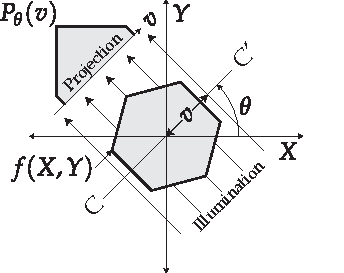
\includegraphics{Chapters/flopt/Figs/PDF/OPT_digram}
  \caption{Principle of OPT, a respective rotation between the sample and the detector illumination pair is iterated, the volumetric image is later reconstructed.}
  \label{fig:OPT_digram}
\end{figure}

\subsection{Reconstruction}

As the sample is rotated each pixel collects an an intensity $I = I_{\theta}e^{-k}$ at discrete angles $n$ through a full rotation of the sample; where $I_{\theta}$ is the unattenuated radiation intensity from the source to the detector, $k$ is the attenuation caused by the sample along a detected ray an $I(\theta)$ is the measured intensity, see Figure %TODO figure
Rays from the sample to the detector approximate straight lines, and so the the rays reaching the detector with a line integrals.
A projection is then the resulting intensity profile at the detector for a rotation angle, and the integral transform that results in $f(I_i,\theta_n)$ is the Radon transform.
This is defined mathematically as:

\begin{align}
    f(I,\theta) = \int \int R(x,y)\delta (xcos(\theta)+y sin(\theta)-I)dx dy
\end{align}

Where $f(I,\theta)$ is the Radon transform, and $R(x,y)$ represents a 2D slice of the sample.
A parallel projection is then just the combination of line integrals $f(I)$ for a constant.% for a constant.
An inverse Radon transform is used to recover the original object from the projection data.
By taking the Fourier transform of each projection measurement and reorder the information from the sample into it's respective place in Fourier space.
This is valid due to the Fourier Slice theorem (%TODO cite
) which states that the Fourier transform of a parallel projection equivalent to a 2D slice of of the Fourier transform original sample.
A spatial filtering step is applied during back-projection to avoid spatial frequency oversampling during the object’s rotation (see Figure %TODO figure 5);
a high pass filter is commonly used to compensate for the percieved blurring.
%A high pass filter such as a ramp filter is commonly used to counter the blurring caused by this oversampling.
FBP be thought of as smearing the projection data across the image plane, and is expressed in equation form as:
\begin{align}
R_{fpb}(x,y) = \int_{0}^{\pi} f'(x\cos(\theta)+y\sin(\theta),\theta)dxdy
\intertext{where $f'$ is the filtered projection data, and $R_{fbp}$ is the back-projected image.}
\end{align} \todo{Verify this?!?!?!}

\subsubsection{Aim}

The Radon transform relies heavily on the assumption of circular motion only.
This chapter hopes to exploit some of the techniques seen in stereoscopic imaging to register back projections rather than relying on line integrals.
The algorithm proposed here is therefore robust to mechanical drifts across acquisitions as well as inconsistent angular .steps

\section{Stereoscopic Imaging}

%\subsection{Projective geometry}

%Camera imaging is governed by projective geometry
%Parallel lines project onto a camera will have a vanishing point at the horizon.

%\subsection{Camera projections}

%\todo{Camera projections \ lecture notes 3}

Imaging scenes in stereo allows for the triangulation of individual points in 3D space, features or fiducials in one detector to another.
Triangulation requires features in both images to be the same, this is known as the correspondence problem.
Many methods exist to ensure that features are known and confidently the same between two cameras; properties of scale independent features and their surrounding pixel environment in one image can be matched to a similar feature in the second image.

Now, suppose we know the relative positions of the two cameras and their intrinsic parameters.
Given the CCD parameters, we can translate pixel coordinates (u, v) into image plane coordinates $(x, y)$:
\begin{align}
    u = u_0 + k_u x \\
    v = v_0 + k_v y
\end{align}

And knowing the focal length of the imaging system, image plane coordinates may be translated into a ray in 3D.
The ray can be defined by a point $\textbf{p}$ in camera-centred coordinates where it crosses the image plane as:

\begin{align}
  \mathbf{p} = \begin{bmatrix}
        x\\y\\z
      \end{bmatrix}
\end{align}

From the definition of a point as observed through an image we can construct a dual-view model of points in space.
Using a model of a system with two views allows for the triangulation of rays based on image correspondences, this is an important part of sterovision.
The most important matching constraint which can be used the \emph{epipolar constraint}, and follows directly from the fact that the rays must intersect in 3D space.
Epipolar constraints facilitate the search for correspondences, they constrain the search to a 1D line in each image.
To derive general epipolar constraints, one should consider the epipolar geometry of two camera as seen in Figure \ref{fig:epi-polar-geom}

The \textbf{baseline} is defined as the line joining the optical centres.
An \textbf{epipole} is the point of intersection of the baseline with the image plan and there are two epipoles, one for each image.
An \textbf{epipolar line} is a line of intersection of the epipolar plane with an image plane.
It is the image in one camera of the ray from the other camera’s optical centre to the point $X$.
For different world points $X$, the epipolar plane rotates about the baseline.
All epipolar lines intersectat the epipole.

The epipolar line constrains the search for correspondence from a region to a line.
If a point feature $\textbf{x}$ is observed in one image, then its location $\textbf{x'}$ in the other image must lie on the epipolar line.
We can derive an expression for the epipolar line.
The two camera-centered coordinate systems are related by a rotation $R$ and translation $\textbf{T}$:

\begin{align}
    \mathbf{X'}_c &= R\mathbf{X'}_c + \mathbf{T} \nonumber \\
    \intertext{Taking the vector product with T, we obtain} \nonumber \\
    T \times \mathbf{X'}_c &= T \times R\mathbf{X'}_c + \mathbf{T} \times \mathbf{T} \nonumber \\
    T \times \mathbf{X'}_c &= T \times R\mathbf{X'}_c \label{Xprime = RTX}
\end{align}

\begin{figure}
  \centering
  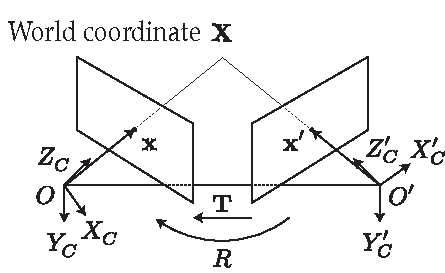
\includegraphics{Chapters/flopt/Figs/PDF/epi-polar-geom}
  \caption{Epi-polar geometry described for two adjacent views (or cameras of a scene).}
  \ref{fig:epi-polar-geom}
\end{figure}

\subsubsection{Essential Matrix}

Taking the scalar product with $\mathbf{X'_c}$, we obtain:
\begin{align}
    \mathbf{X'}_c \cdot (\mathbf{T} \times \mathbf{X'}_c) &= \mathbf{X'}_c\cdot (\mathbf{T} \times R\mathbf{X'}_c)\nonumber \\
    \mathbf{X'}_c \cdot (\mathbf{T} \times R\mathbf{X'}_c) &= 0 \nonumber
\end{align}
A vector product can be expressed as a matrix multiplication:
\begin{align}
T \times \mathbf{X}_c &= T_\times \mathbf{X}_c \\
\intertext{where}
T_\times &=\begin{bmatrix}
0    & -T_z  & T_y\\
T_z  & 0     & -T_x\\
-T_y  & T_x   & 0
\end{bmatrix}
\end{align}
So equation \eqref{eq:Xprime = RTX} can be rewritten as:

\begin{align}
\mathbf{X'}_c \cdot (T_\times R\mathbf{X}_c) = 0 \nonumber\\
\mathbf{X'}_c T E \mathbf{X}_c = 0  \nonumber\\
\intertext{where}  \nonumber\\
E = T_\times R \nonumber
\end{align}

E is a $3 \times 3$ matrix known as the \emph{essential matrix}.
The constraint also holds for rays $\mathbf{p}$, which are parallel to the camera-centered position vectors $\mathbf{X}_c$:

\begin{align}
\mathbf{p}'^T E \mathbf{p} = 0 \label{eq:pEp}
\end{align}
This is the epipolar constraint.
If we observe a point $\mathbf{p}$ in one image, then its position $\mathbf{p'}$ in the other image must lie on the line defined by \eqref{eq:pEp}.
The essential matrix can convert from pixels on the detector to rays $\mathbf{p}$, assuming a calibrated camera.
And pixel coordinates can then be converted to image plane coordinates using:
\begin{align}
\begin{bmatrix}
u\\
v\\
1
\end{bmatrix}
&=
\begin{bmatrix}
k_u & 0 & u_0 \\
0 & k_v & v_0 \\
0 & 0 & 1
\end{bmatrix}
\begin{bmatrix}
x\\
y\\
1
\end{bmatrix}
\intertext{We can modify this to derive a relationship between pixel coordinates and rays:}
\begin{bmatrix}
u\\
v\\
1
\end{bmatrix}
&=
\begin{bmatrix}
\frac{k_u}{f} & 0 & \frac{u_0}{f} \\
0 & \frac{k_v}{f} & \frac{v_0}{f} \\
0 & 0 & \frac{1}{f}
\end{bmatrix}
\begin{bmatrix}
x\\
y\\
f
\end{bmatrix}
\intertext{If we define the matrix $K$ as follows:}
K &= \begin{bmatrix}
f k_u & 0 & u_0 \\
0 & f k_v & v_0 \\
0 & 0 & 1
\end{bmatrix}
\intertext{then we can write}
\mathbf{\widetilde{w}} &= K\mathbf{p}
\end{align}

\subsubsection{Fundamental Matrix}

\begin{align}
    \intertext{The epipolar constraint becomes}\\
    \mathbf{p'}^T E \mathbf{p} &= 0 \\
    \mathbf{\widetilde{w'}}^T K^{-T} E K^{-1} \mathbf{\widetilde{w}} &= 0 \\
    \mathbf{\widetilde{w'}}^T F \mathbf{\widetilde{w}} &= 0
\end{align}

F is the $3\times3$ \emph{fundamental matrix}.

%\subsubsection{Two views}
%\paragraph{Mapping from one camera to another}
%\subsubsection{Three and more views}

With intrinsically calibrated cameras, structure can be recovered by triangulation.
Firstly the two projection matrices are obtained via a singular value decomposition of the essential matrix.
The SVD of the essential matrix is given by:

\begin{align}
    \hat{T}_{\times} = U \begin{bmatrix}
    0 & 1 & 0 \\
    -1 & 0 & 0 \\
    0 & 0 & 0
    \end{bmatrix} U^T
    &\text{ and }
    R = U \begin{bmatrix}
    0 & -1 & 0 \\
    1 & 0 & 0 \\
    0 & 0 & 1
    \end{bmatrix} V^T
    \intertext{Then, aligning the left camera and world coordinate
    systems:}
    P = K [I | \mathbf{0}]
    &\text{ and }
    P' = ' [R | \mathbf{T}]
\end{align}

Given the two projection matrices, we can recover structure (only up to scale, since $|\mathbf{T}|$ is unknown) using least squares.
Ambiguities in $\mathbf{T}$ and R are resolved by ensuring that visible points lie in front of the two cameras.
As with the essential matrix, the fundamental matrix can be factorised into a skew-symmetric matrix corresponding
to translation and a 3 × 3 non-singular matrix corresponding to rotation.

\section{The proposed algorithm}

%The rotation may also not be orthogonal to the plane of detection.
During a typical OPT acquisition, a fiducial will appear to follow an elliptical path in $xy$.
In the following volume reconstruction there will then be a fitting step to recover the path of the fiducial, to then apply a correction before applying a radon transform.
This type of reconstruction not only ignores any mechanical jitter of the sample but also any systematic drift.

We have seen that using two adjacent images of a scene separated by some rotation and translation, points in 3D space may be triangulated within the scene given the rotational and translational matrices of the respect camera views.
The inverse is also possible, given a sufficient amount of reliable known fiducial points in a scene the translation and rotation matrices can be recovered.
The recovery over a more exact description of the motion of the scene can eliminate any need for a fitting and may recover and correct for drift as well as eliminate any mechanical jitter.
Errors may however then be introduced from fiducials mechanically slipping and localisation errors.
The shift of a camera or a camera pair around a scene separated by a translation matrix is analogous to a sample moving in in the fixed view of an imaging detector, like in OPT.

Once a sufficient amount of fidicuials are reliably tracked from the first to the second image, the Fundamental, Essential or Homography can be computed.
Using the factorisation one of these matrixes between each adjacent view of a rotating scene the translation and rotational matrices may be recovered.
Here we will discuss a reconstruction using $F$ but the same principle applies for $E$ and $H$.

\begin{figure}
  \centering
  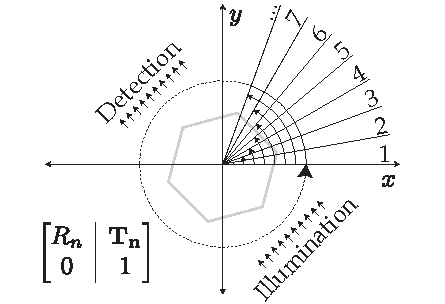
\includegraphics{Chapters/flopt/Figs/PDF/flOPT_principle}
  \caption{Each iteration during an OPT acquisition will have an associate $R$ and $\mathbf{T}$, these matrices can be recovered from comparing the current iteration to the previously iteration.}
\end{figure}

Here are two ways of reconstructing using the Fundamental matrix as described above.
The first method involves computing F for two neighbouring images with 5 or more fiducials, having more beads helps to remove ambiguity and increase confidence in F.
Once F is calculated F is then decomposed into $R_n$ and $T_n$ between each view $n$ and $n+1$.
The image at view $n+1$ is then back projected along the virtual optical axis within a virtual volume where the sample will be reconstructed.
The size of this back projection and virtual volume is chosen to be suitably large (so that important data is not lost).
Then, all the prior rotation and translation matrices are serially multiplied from $[R_0|T_0]$ until $[R_n|T_n]$, this final matrix is inverted and applied to the back projected volume.
The matrix inversion step is important as it realigns the back projection in the volume to where it originally was compared respective of the first projection.
This process is repeated for every angle and the back projected volume from each step is summed with every other step.
Finally the remaining volume is filtered using a high-pas filter, here a Ram-Lak filter is used.
\footnote{Linear ramp filter in Fourier space: $|v|$},
By producing a series of transformation matrices from adjacent acquisitions, errors compound and the reconstruction of volumes degrades with more projections, see Figure \ref{fig:irandons}.

\begin{figure}
  \centering
  \hfill
  \begin{subfigure}[t]{0.3\textwidth}
    
\includegraphics[width=\textwidth]{Chapters/flopt/Figs/PDF/results/no_helix/iradon_nofilter}
    \caption{Unfiltered output of the radon transform}
    \label{fig:iradon_nofilter}
  \end{subfigure}\hfill
  \begin{subfigure}[t]{0.3\textwidth}
    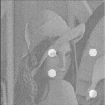
\includegraphics[width=\textwidth]{Chapters/flopt/Figs/PDF/results/no_helix/iradon_filter}
    \caption{Ram-lak (Fourier ramp) filter applied to Figure \ref{fig:iradon_nofilter}.}
    \label{fig:iradon_filter}
  \end{subfigure}
    \hfill
    \label{fig:irandons}
  \caption{The result of an Tomographic reconstruction requires Fourier filtering to normalise spatial contrast}
\end{figure}

The following approach is less prone to compound errors but relies on precise fiducial distinction and tracking.
Instead of calculating F between neighbouring images F is calculated between the current projection and the very first projection.
F is then decomposed and the transformation matrix is inverted and applied to the back projected volume.
The reoriented back projected volumes are summed and finally filtered to remove the additional spatial frequencies imparted from rotating the sample.

\begin{figure}
  \centering
  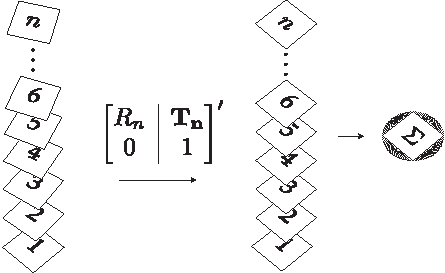
\includegraphics{Chapters/flopt/Figs/PDF/flopt_algorithm}
  \caption{Two dimensional representation of the reconstruction algorithm.
  The rotational and translation matrices are recovered and inversely applied to back projected images.
  The now realigned back projection are summated to produce an unfiltered back projection.}
\end{figure}

The second approach may be robust to compound errors but an additional programatic step is needed to know which beads in the first image correspond to beads in the current image.
This can be is achieved using standard tracking and momentum particle tracking algorithms.
In both cases a decomposed F will produce four possible transformation pairs. %(R,T; R,-T; -R,T; -R,-T) %TODO look this up.
Once the transformation matrix between the first view and the second view is calculated the proceeding transformation matrices are then easily chosen by similarity and general direction of motion.
An example of this type of selection would be:
\begin{align}
\min_{I(n)}I(n) = ([R_n|T_n]  - [R_{n-1}|T{n-1}])^2
\end{align}
The first two views are more difficult to choose the correct decomposition form but it is possible if a suitable ideal matrix is given as a comparison.
Such an ideal matrix is composed using \emph{a priori} knowledge of the likely angle of rotation of the system's imaging properties.

\section{Results}

To verify the proposed algorithm successfully reconstructs as theorised, it was applied to simulated data.
The image of Lena
\footnote{The image of Lena is used as a reference to a very early full colour digital scanner.
The researchers in question realised that their presentation of the scanner's capabilities at a conference lacked a test image.
The nearest image to hand was a Playboy magazine with Lena Söderberg as the centrefold.}
is used here as a test image to verify the validity of each reconstruction.
Superimposed on Lena are fiducial beads to track the rotation of the image, see Figure \ref{fig:raw_input}.
The reference image was then rotated through 128 angles over $2\pi$ radians and projected along the $y$ axis and a slice in $xy$ was taken to create a single line projection.
This is repeated for each angle with each line projection stacked to create a sinugram, see Figure \ref{fig:sinugram_stretch}.

\begin{figure}
  \centering
  \hfill
  \begin{subfigure}[t]{0.3\textwidth}
    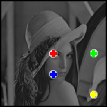
\includegraphics[width=\textwidth]{Chapters/flopt/Figs/PDF/results/no_helix/rawinput_colour}
    \caption{Raw input for OPT simulations, Lena.}
    \label{fig:raw_input}
  \end{subfigure}\hfill
  \begin{subfigure}[t]{0.3\textwidth}
    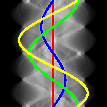
\includegraphics[width=\textwidth]{Chapters/flopt/Figs/PDF/results/no_helix/sinugram_stretch}
    \caption{Image of Lena (Figure \ref{fig:raw_input}) after rotation and projection in 2D, giving the sinugram.}
    \label{fig:sinugram_stretch}
  \end{subfigure}
  \hfill
  \label{fig:rawinputs}
  \caption{Reference images for OPT reconstruction.}
\end{figure}

\begin{figure}
  \centering
  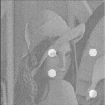
\includegraphics[width=0.3\textwidth]{Chapters/flopt/Figs/PDF/results/no_helix/flopt_filter}
\caption{Reconstruction of a reference image using the new proposed algorithm}
\label{fig:flopt_filter}
\end{figure}

In the standard algorithmic approach for OPT, the sinugram produced then undergoes the Radon transform, see Figure \ref{fig:iradon_nofilter} and then a post filtering, see Figure \ref{fig:iradon_nofilter}.
This step is substituted for the proposed algorithm; in Figure \ref{fig:flopt_comparison_line_profile} the two techniques are compared for ideal conditions of smooth, predictable rotation.
The proposed algorithm produces (see Figure \ref{fig:flopt_filter}) a faithful reconstruction on the original image, with some minor deviations.
Both techniques lose some of the original contrast of the image due to under-sampling of rotations.
When taking the histogram of the absolute pixel-wise difference between the original source image to the images produced by the new algorithm and the Radon transform, there is a clear shift to less discrepant pixels for the new algorithm.
This would suggest that the new algorithm is producing a more accurate interpretation than the standard radon transform, see Figure \ref{fig:flopt_histogram}

\begin{figure}
  \centering
  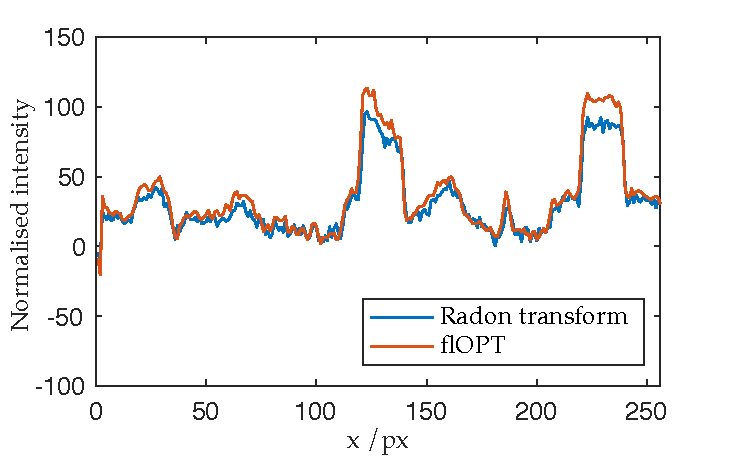
\includegraphics{Chapters/flopt/Figs/PDF/results/comparison_line_profile}
  \caption{Line profile comparison of the reconstruction of a reference image artificially rotated and projected using the standard radon transform and the new proposed algorithm.}
  \label{fig:flopt_comparison_line_profile}
\end{figure}

\begin{figure}
  \centering
  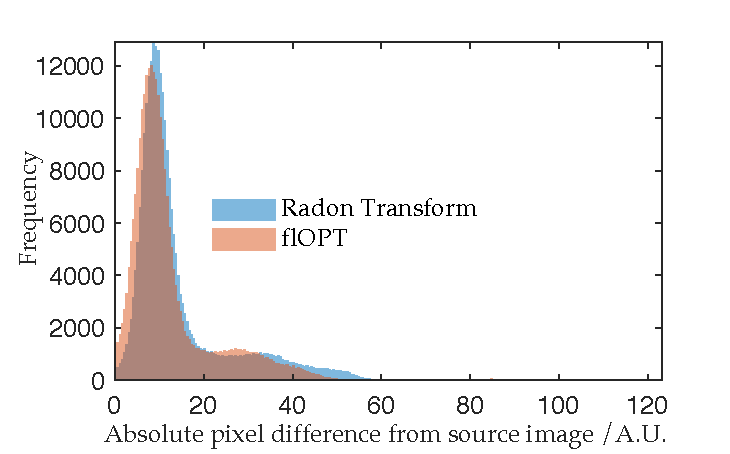
\includegraphics{Chapters/flopt/Figs/PDF/results/flopt_histogram}
  \caption{Histogram of of pixel values compared between reconstructions using flOPT and the Radon transform.
  The shift of the histogram to towards overall lower deviance from the source image suggests the flOPT algorithm out performs the radon transform}
  \label{fig:flopt_histogram}
\end{figure}

%However, the proposed algorithm fairs worse in terms of contrast compared to a Radon transform.

The more challenging case of a sample drifting systematically along the $x$ axis was then considered, this produced a helical path of a single fiducial within the sample, see Figure\ref{fig:flopt_helix_sinugram}.
In Figure \ref{fig:unfilttered_reconstruction_helix_iradon} the Radon transform entirely fails to produce a recognisable reproduction of the test image with the addition of a slight helicity to the rotation.
The proposed algorithm produces an equivalent result to that of a sample rotating without any systematic drift, see Figure \ref{fig:iradon_filter}.
In Figure \ref{fig:helical_comparison} the respective images from each algorithm were compared as before while the helical shift was incremented.
See Figure \ref{fig:flopt_helix_sinugram} for a sinugram of a sample whereby a helical shift has been induced.
When using correlation as a metric of reproduction quality, at zero helicity, the new algorithm fairs slightly worse at 94\% correlation compared to the Radon transform at 96\%.
As expected, the Radon transform rapidly deteriorates once a systematic drift is applied; where-as the new algorithm maintains quality of reconstruction, see Figure \ref{fig:helical_comparison}.

\begin{figure}
  \centering
  \hfill
  \begin{subfigure}[t]{0.3\textwidth}
    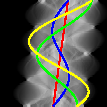
\includegraphics[width=\textwidth]{Chapters/flopt/Figs/PDF/results/helix/sinugram_stretch}
    \caption{Sinugram of a sample whose axis of rotation has a systematic drift}
    \label{fig:flopt_helix_sinugram}
  \end{subfigure}\hfill
  \begin{subfigure}[t]{0.3\textwidth}
    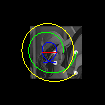
\includegraphics[width=\textwidth]{Chapters/flopt/Figs/PDF/results/helix/topdown_bead_paths}
    \caption{Top down ($xy$) of source image with fiducial paths marked.}
    \label{fig:topdown_bead_paths}
  \end{subfigure}
    \hfill
    \label{fig:flopts}
  \caption{Comparison of the two reconstructions under sample imaging with a systematic drift, in 3D though represented here in 2D.}
\end{figure}
\begin{figure}
  \centering
  \hfill
  \begin{subfigure}[t]{0.3\textwidth}
    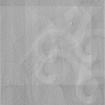
\includegraphics[width=\textwidth]{Chapters/flopt/Figs/PDF/results/helix/unfilttered_reconstruction_helix_iradon}
    \caption{Unfiltered reconstruction using a radon transform}
    \label{fig:unfilttered_reconstruction_helix_iradon}
  \end{subfigure}\hfill
  \begin{subfigure}[t]{0.3\textwidth}
    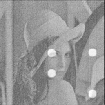
\includegraphics[width=\textwidth]{Chapters/flopt/Figs/PDF/results/helix/filtered_recon_helix}
    \caption{Filtered reconstruction using the new algorithm}
    \label{fig:filtered_recon_helix}
  \end{subfigure}
    \hfill
    \label{fig:flopts}
  \caption{Comparison of the two reconstructions under sample imaging with a systematic drift, in 3D though represented here in 2D.}
\end{figure}
\begin{figure}
  \centering
  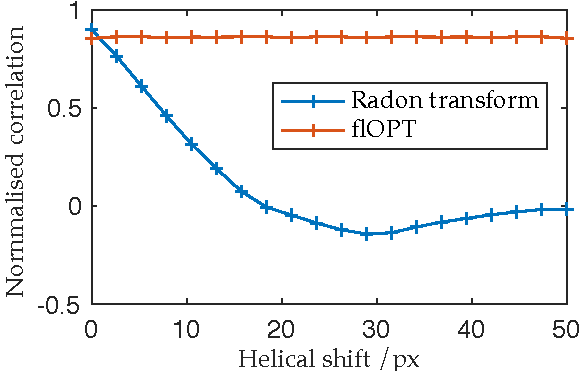
\includegraphics{Chapters/flopt/Figs/PDF/results/correlation_helicity}
  \caption{2D correlation of the source image shows that flOPT does not degrade under systematic drift compared to Radon Transforms.}
  \label{fig:helical_comparison}
\end{figure}


\subsubsection{Recovery of R and T using matrix decomposition}

To quantitatively verify that the matrix decomposition technique was valid and robust, the accuracy of the reproduction of $R$ and $\mathbf{T}$ was tested directly.
The the original $R$ and $\mathbf{T}$ matrices were computed and compared to $R$ and $\mathbf{T}$ generated from matrix decomposition, this absolute difference was computed element-wise in each matrix and then an average for each matrix was taken.
Overall the worst case scenario produced a percentage error of $2\%$ see Figure \ref{fig:pc_sum_decompose} for full statistics.
The accuracy of the calculated $R$ and $\mathbf{T}$ did deteriorate when adding in additional degrees of combined movement, but the severity of this movement appeared to no trending effect.
Consistently the translational matrix was more accurately reproduced, this is likely due to there being fewer of degrees of freedom for errors to spread over.

%The images produced are a more faithful reproduction of the source image as the degree of helicity is increased.
%This effect may be due to the additional sampling induced by adding another degree of movement, that is the systematic drift.

%Textwidth is \the\textwidth


\begin{figure}
  \centering
    \begin{subfigure}[t]{0.5\textwidth}
      \captionsetup{width=0.8\textwidth}
      \centering
      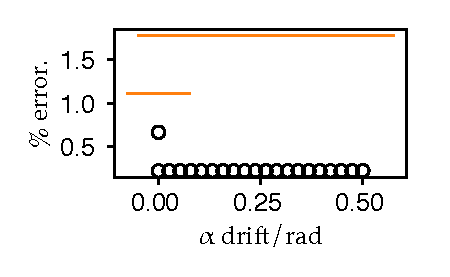
\includegraphics{Chapters/flopt/Figs/PDF/results/helix/decompose/pc_sum_rot_alpha}
      \caption{Rotation matrix, with angular drift in $\alpha$}\label{fig:pc_sum_rot_alpha}
    \end{subfigure}\hfill
    \begin{subfigure}[t]{0.5\textwidth}
      \captionsetup{width=0.8\textwidth}
      \centering
      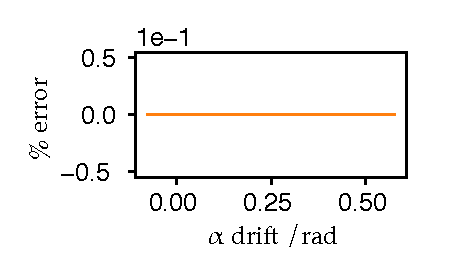
\includegraphics{Chapters/flopt/Figs/PDF/results/helix/decompose/pc_sum_trans_alpha}
      \caption{Translation matrix, with angular drift in $\alpha$}\label{fig:pc_sum_trans_alpha}
    \end{subfigure}
    \bigskip
        \begin{subfigure}[t]{0.5\textwidth}
          \captionsetup{width=0.8\textwidth}
          \centering
          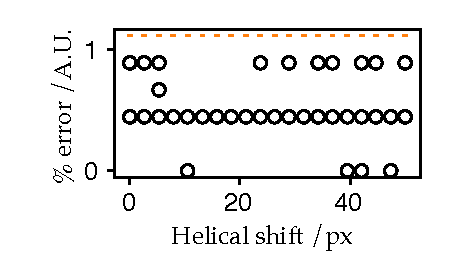
\includegraphics{Chapters/flopt/Figs/PDF/results/helix/decompose/pc_sum_rot_tx}
          \caption{Rotation matrix, with helical drift in $x$ only}\label{fig:pc_sum_rot_tx}
        \end{subfigure}\hfill
        \begin{subfigure}[t]{0.5\textwidth}
          \captionsetup{width=0.8\textwidth}
          \centering
          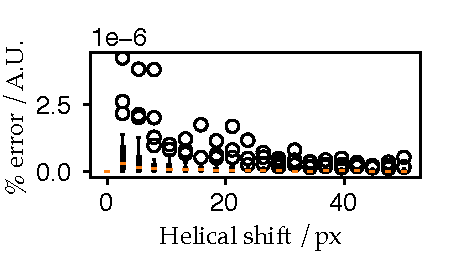
\includegraphics{Chapters/flopt/Figs/PDF/results/helix/decompose/pc_sum_trans_tx}
          \caption{Translation matrix, with helical drift in $x$ only} \label{fig:pc_sum_trans_tx}
        \end{subfigure}
    \bigskip
        \begin{subfigure}[t]{0.5\textwidth}
          \captionsetup{width=0.8\textwidth}
          \centering
          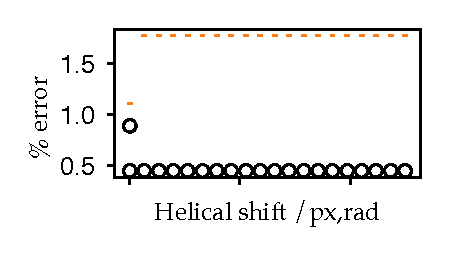
\includegraphics{Chapters/flopt/Figs/PDF/results/helix/decompose/pc_sum_rot_both}
          \caption{Rotation matrix, with angular drift in $\alpha$ and helical drift in $x$}\label{fig:pc_sum_rot_both}
        \end{subfigure}\hfill
        \begin{subfigure}[t]{0.5\textwidth}
          \captionsetup{width=0.8\textwidth}
          \centering
          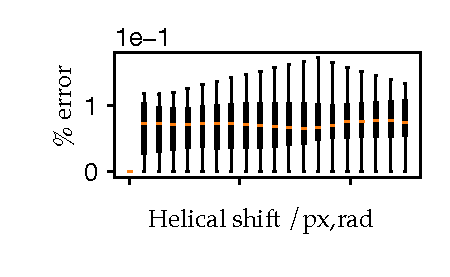
\includegraphics{Chapters/flopt/Figs/PDF/results/helix/decompose/pc_sum_trans_both}
          \caption{Translation matrix, with angular drift in $\alpha$ and helical drift in $x$}\label{fig:pc_sum_trans_both}
        \end{subfigure}
          \caption{Box plots demonstrating that the Rotational and Translations matrices can be recovered accurately from fiducial marker positions.
          Panels \ref{fig:pc_sum_rot_alpha} and \ref{fig:pc_sum_trans_alpha} introduce an angular drift during rotation, to an observer at the detector this would appear as a tip of the sample towards them, causing precession.
          Panels \ref{fig:pc_sum_rot_tx} and \ref{fig:pc_sum_trans_tx} introduce a lateral drift in $x$ causing a helical path to be drawn out.
          Panels \ref{fig:pc_sum_rot_both} and \ref{fig:pc_sum_trans_both} combine the two effects.
          In all cases the percentage error introduced by the the addition of undesirable additional movements was on the order of $<2\%$.
          }
          \label{fig:pc_sum_decompose}
\end{figure}

\section{Discussion}

A new algorithm for reconstructing OPT data has been demonstrated.
The new algorithm uses multiple fiducials to recover the matrix which describes the rotation and translation.
The quality of the reconstructions when compared to a standard radon transform shows a slight improvement, with a great effect when a systematic drift is introduced.
When  comparing the expected matrices to the recovered matrices a peak of $2\%$ difference is found between the two when considering worst case scenarios; suggesting the technique is robust to all forms of drift and general instability.
Such an algorithm could be used to help in minimising ghosting effects seen in real samples; particularly in samples where slipping is likely to occur such as in gels or in cheaper OPT systems which tend to be more mechanically unstable and imprecise.

\subsection{Future work}

\subsubsection{Bead Tracking}
The work presented here is, so far, is only proof-of-concept and requires several steps in order apply it to real OPT data.
Firstly, a full bead tracking algorithm will need to be created to track multiple beads concurrently in an image series.
A sensible approach would be to have a user select the fiducials in the image on the first frame and template match in a small window around the selection; this is similar to the algorithm described in Chapter %TODO insert chapter
Template matching is robust to occlusions provided the fidcuial is not fully eclipsed.
If two fiducials occlude each other however, this algorithm may switch their identities or both tracking windows may follow one bead.
This is a common problem in particle tracking algorithms but is essentially solved by using a weighted likelihood based on momentum.

The likelihood of a bead occlusion occurring will increase with he introduction of additional beads into the sample.
As such occluded beads may need to be omitted and possibly interpolated for.
Egregious outliers may be found by tracking a \emph{confidence} estimator as the bead rotates.
A primitive estimator would be the pixel-wise sum of intensities in the result of a correlative template matching.
Whilst this confidence value itself has no physical interpretation, any stark changes in the derivative will be suggestive of an occlusion or mis-tracking of some variety, see Figure \ref{fig:confidence_bead_tracking}.

\begin{figure}
  \centering
  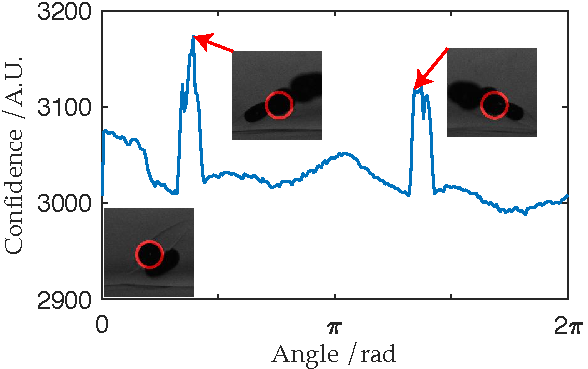
\includegraphics{Chapters/flopt/Figs/PDF/results/confidence_bead_tracking}
  \caption{A plot of the confidence value of a single fiducial bead being tracking \emph{in vivo}.
  Sharp changes in the confidence value occur when the fiducial bead is occluded.
  The image at the origin shows the fiducial being tracked well in the first frame.
  (Images courtesy of Pedro Vallejo)
  }
  \label{fig:confidence_bead_tracking}
\end{figure}

\subsubsection{Multiple Views Tracking}
The theory backing the proposed algorithm relies on triangulation between two view points.
However, it is possible to use three separate views to reconstruct a scene, one such approach being used quaternion tensors.
Working with tensors is computationally and mathematically more challenging, but a future iteration of the algorithm presented here may benefit from using three views to provide a more accurate transformation matrix.
Beyond three views there currently is no mathematical framework at present for four or more views.
If such tools did exist, it may be possible to make the algorithm described above as non-iterative and essentially a single shot reconstruction from pixels to voxels.

%A future version of this algorithm may be able to use 3 views to produce a more faithful transformation matrix.
%The mathematics for more than three views currently does not exist.
